%%
%% Beginning of file 'sample61.tex'
%%
%% Modified 2016 September
%%
%% This is a sample manuscript marked up using the
%% AASTeX v6.1 LaTeX 2e macros.
%%
%% AASTeX is now based on Alexey Vikhlinin's emulateapj.cls 
%% (Copyright 2000-2015).  See the classfile for details.

%% AASTeX requires revtex4-1.cls (http://publish.aps.org/revtex4/) and
%% other external packages (latexsym, graphicx, amssymb, longtable, and epsf).
%% All of these external packages should already be present in the modern TeX 
%% distributions.  If not they can also be obtained at www.ctan.org.

%% The first piece of markup in an AASTeX v6.x document is the \documentclass
%% command. LaTeX will ignore any data that comes before this command. The 
%% documentclass can take an optional argument to modify the output style.
%% The command below calls the preprint style  which will produce a tightly 
%% typeset, one-column, single-spaced document.  It is the default and thus
%% does not need to be explicitly stated.
%%
%%
%% using aastex version 6.1
\documentclass[twocolumn]{aastex61}

%% The default is a single spaced, 10 point font, single spaced article.
%% There are 5 other style options available via an optional argument. They
%% can be envoked like this:
%%
%% \documentclass[argument]{aastex61}
%% 
%% where the arguement options are:
%%
%%  twocolumn   : two text columns, 10 point font, single spaced article.
%%                This is the most compact and represent the final published
%%                derived PDF copy of the accepted manuscript from the publisher
%%  manuscript  : one text column, 12 point font, double spaced article.
%%  preprint    : one text column, 12 point font, single spaced article.  
%%  preprint2   : two text columns, 12 point font, single spaced article.
%%  modern      : a stylish, single text column, 12 point font, article with
%% 		  wider left and right margins. This uses the Daniel
%% 		  Foreman-Mackey and David Hogg design.
%%
%% Note that you can submit to the AAS Journals in any of these 6 styles.
%%
%% There are other optional arguments one can envoke to allow other stylistic
%% actions. The available options are:
%%
%%  astrosymb    : Loads Astrosymb font and define \astrocommands. 
%%  tighten      : Makes baselineskip slightly smaller, only works with 
%%                 the twocolumn substyle.
%%  times        : uses times font instead of the default
%%  linenumbers  : turn on lineno package.
%%  trackchanges : required to see the revision mark up and print its output
%%  longauthor   : Do not use the more compressed footnote style (default) for 
%%                 the author/collaboration/affiliations. Instead print all
%%                 affiliation information after each name. Creates a much
%%                 long author list but may be desirable for short author papers
%%
%% these can be used in any combination, e.g.
%%
%% \documentclass[twocolumn,linenumbers,trackchanges]{aastex61}

%% AASTeX v6.* now includes \hyperref support. While we have built in specific
%% defaults into the classfile you can manually override them with the
%% \hypersetup command. For example,
%%
%%\hypersetup{linkcolor=red,citecolor=green,filecolor=cyan,urlcolor=magenta}
%%
%% will change the color of the internal links to red, the links to the
%% bibliography to green, the file links to cyan, and the external links to
%% magenta. Additional information on \hyperref options can be found here:
%% https://www.tug.org/applications/hyperref/manual.html#x1-40003

%% If you want to create your own macros, you can do so
%% using \newcommand. Your macros should appear before
%% the \begin{document} command.
%%
\newcommand{\vdag}{(v)^\dagger}
\newcommand\aastex{AAS\TeX}
\newcommand\latex{La\TeX}
\newcommand{\sm}{M_\odot}
\newcommand{\sr}{R_\odot}

%% Reintroduced the \received and \accepted commands from AASTeX v5.2
\received{\today}
\revised{\today}
\accepted{\today}
%% Command to document which AAS Journal the manuscript was submitted to.
%% Adds "Submitted to " the arguement.
\submitjournal{ApJ}

%% Mark up commands to limit the number of authors on the front page.
%% Note that in AASTeX v6.1 a \collaboration call (see below) counts as
%% an author in this case.
%
%\AuthorCollaborationLimit=3
%
%% Will only show Schwarz, Muench and "the AAS Journals Data Scientist 
%% collaboration" on the front page of this example manuscript.
%%
%% Note that all of the author will be shown in the published article.
%% This feature is meant to be used prior to acceptance to make the
%% front end of a long author article more manageable. Please do not use
%% this functionality for manuscripts with less than 20 authors. Conversely,
%% please do use this when the number of authors exceeds 40.
%%
%% Use \allauthors at the manuscript end to show the full author list.
%% This command should only be used with \AuthorCollaborationLimit is used.

%% The following command can be used to set the latex table counters.  It
%% is needed in this document because it uses a mix of latex tabular and
%% AASTeX deluxetables.  In general it should not be needed.
%\setcounter{table}{1}

%%%%%%%%%%%%%%%%%%%%%%%%%%%%%%%%%%%%%%%%%%%%%%%%%%%%%%%%%%%%%%%%%%%%%%%%%%%%%%%%
%%
%% The following section outlines numerous optional output that
%% can be displayed in the front matter or as running meta-data.
%%
%% If you wish, you may supply running head information, although
%% this information may be modified by the editorial offices.
\shorttitle{iPTF16abc}
\shortauthors{Cao et al.}
%%
%% You can add a light gray and diagonal water-mark to the first page 
%% with this command:
\watermark{DRAFT}
%% where "text", e.g. DRAFT, is the text to appear.  If the text is 
%% long you can control the water-mark size with:
%  \setwatermarkfontsize{dimension}
%% where dimension is any recognized LaTeX dimension, e.g. pt, in, etc.
%%
%%%%%%%%%%%%%%%%%%%%%%%%%%%%%%%%%%%%%%%%%%%%%%%%%%%%%%%%%%%%%%%%%%%%%%%%%%%%%%%%

%%%%%%%%%%%%%%%%%%%%%%%%%%%%%%%%%%%%%%%%%%%%%%%%%%%%%%%%%%%%%%%%%%%%%%%%%%%%%%%%
%%
%% The following section defines new commands for comments from co-authors
%%
\newcommand{\ycao}[1]{{\color{red} ycao: {#1}}}
%%
%%%%%%%%%%%%%%%%%%%%%%%%%%%%%%%%%%%%%%%%%%%%%%%%%%%%%%%%%%%%%%%%%%%%%%%%%%%%%%%%

%% This is the end of the preamble.  Indicate the beginning of the
%% manuscript itself with \begin{document}.

\begin{document}

\title{iPTF16abc}

%% LaTeX will automatically break titles if they run longer than
%% one line. However, you may use \\ to force a line break if
%% you desire. In v6.1 you can include a footnote in the title.

%% A significant change from earlier AASTEX versions is in the structure for 
%% calling author and affilations. The change was necessary to implement 
%% autoindexing of affilations which prior was a manual process that could 
%% easily be tedious in large author manuscripts.
%%
%% The \author command is the same as before except it now takes an optional
%% arguement which is the 16 digit ORCID. The syntax is:
%% \author[xxxx-xxxx-xxxx-xxxx]{Author Name}
%%
%% This will hyperlink the author name to the author's ORCID page. Note that
%% during compilation, LaTeX will do some limited checking of the format of
%% the ID to make sure it is valid.
%%
%% Use \affiliation for affiliation information. The old \affil is now aliased
%% to \affiliation. AASTeX v6.1 will automatically index these in the header.
%% When a duplicate is found its index will be the same as its previous entry.
%%
%% Note that \altaffilmark and \altaffiltext have been removed and thus 
%% can not be used to document secondary affiliations. If they are used latex
%% will issue a specific error message and quit. Please use multiple 
%% \affiliation calls for to document more than one affiliation.
%%
%% The new \altaffiliation can be used to indicate some secondary information
%% such as fellowships. This command produces a non-numeric footnote that is
%% set away from the numeric \affiliation footnotes.  NOTE that if an
%% \altaffiliation command is used it must come BEFORE the \affiliation call,
%% right after the \author command, in order to place the footnotes in
%% the proper location.
%%
%% Use \email to set provide email addresses. Each \email will appear on its
%% own line so you can put multiple email address in one \email call. A new
%% \correspondingauthor command is available in V6.1 to identify the
%% corresponding author of the manuscript. It is the author's responsibility
%% to make sure this name is also in the author list.
%%
%% While authors can be grouped inside the same \author and \affiliation
%% commands it is better to have a single author for each. This allows for
%% one to exploit all the new benefits and should make book-keeping easier.
%%
%% If done correctly the peer review system will be able to
%% automatically put the author and affiliation information from the manuscript
%% and save the corresponding author the trouble of entering it by hand.

\correspondingauthor{Yi Cao}
\email{ycao16@uw.edu}

\author[0000-0002-8036-8491]{Yi Cao}
\affil{eScience Institute and Astronomy Department, University of Washington,
  Seattle, WA 98195}

\author{Friends}
\affil{the intermediate Palomar Transient Factory}

%% Note that the \and command from previous versions of AASTeX is now
%% depreciated in this version as it is no longer necessary. AASTeX 
%% automatically takes care of all commas and "and"s between authors names.

%% AASTeX 6.1 has the new \collaboration and \nocollaboration commands to
%% provide the collaboration status of a group of authors. These commands 
%% can be used either before or after the list of corresponding authors. The
%% argument for \collaboration is the collaboration identifier. Authors are
%% encouraged to surround collaboration identifiers with ()s. The 
%% \nocollaboration command takes no argument and exists to indicate that
%% the nearby authors are not part of surrounding collaborations.

%% Mark off the abstract in the ``abstract'' environment. 
\begin{abstract}

  In this paper, we present observations of a young normal Type Ia supernova
  iPTF16abc. Our analysis shows that: blabla ...

\end{abstract}

%% Keywords should appear after the \end{abstract} command. 
%% See the online documentation for the full list of available subject
%% keywords and the rules for their use.
\keywords{methods: observational --- supernovae: individual (iPTF16abc)}

%% From the front matter, we move on to the body of the paper.
%% Sections are demarcated by \section and \subsection, respectively.
%% Observe the use of the LaTeX \label
%% command after the \subsection to give a symbolic KEY to the
%% subsection for cross-referencing in a \ref command.
%% You can use LaTeX's \ref and \label commands to keep track of
%% cross-references to sections, equations, tables, and figures.
%% That way, if you change the order of any elements, LaTeX will
%% automatically renumber them.

%% We recommend that authors also use the natbib \citep
%% and \citet commands to identify citations.  The citations are
%% tied to the reference list via symbolic KEYs. The KEY corresponds
%% to the KEY in the \bibitem in the reference list below. 

\section{Introduction}
\label{sec:intro}

Although Type Ia supernovae (SNe Ia) have been extensively used as
standardizable candles, their progenitor scenarios and explosion
physics are still in debate (see a recent review by
\citealt{2014ARA&A..52..107M}). Detailed extermely early-phase
observations are one of the most promising avenues to further
constrain this problem.

While the shock breakout of a SN Ia occurs on a sub-second timescale,
the subsequent quasi-adiabatic expanding and cooling of the unbinded
ejecta produces thermal emissions that can be used to infer the
original size of the exploding star
\citep{2010ApJ...708..598P,2011ApJ...728...63R}. Comparing models of
these cooling emissions to the earliest-phase data of SN2011fe,
\citet{2012ApJ...744L..17B} concluded that the radius of the
progenitor star is $\lesssim0.01\sr$ where $\sr$ is the solar
radius. Combining this size constraint and the measured ejecta mass to
derive the mean density of the progenitor star, we confirmed that the
progenitor star is compact and degenerate. Admittedly, due to the
initial small surface area of the progenitor star, the shock cooling
emission of a SN Ia decays drastically as the ejecta expands. Given
typical parameters of a SN Ia, this thermal emission is visible from
events up to $\sim 10\,\textrm{Mpc}$ within one day of their explosions.

Another expectation from the extremely early-phase observations of a
SN Ia is the excess emission from collisions between SN ejecta and a
companion star, a natural consequence from the single-degenerate
progenitor hypothesis \citep{1973ApJ...186.1007W,2010ApJ...708.1025K}.
In a low-velocity SN Ia iPTF14atg, \citet{2015Natur.521..328C} for the
first time detected a strong and declining ultraviolet pulse within a
few days of the SN explosion which is best interpreted as the
SN-companion collision. This signature has been searched in a number
of nearby, early-phase normal SNe Ia, but most of these studies result
in no detection
\citep{2010ApJ...722.1691H,2011ApJ...741...20B,2012ApJ...744...38F,
  2012ApJ...744L..17B,2015Natur.521..332O,
  2013ApJ...778L..15Z,2015ApJ...799..106G,2016ApJ...826..144S,
  2015ApJS..221...22I}. The exception is SN2012cg which
\citet{2016ApJ...820...92M} claimed detection of blue excess in the
earliest-phase light curve and attribute it to SN-companion collision.
However, this statement is recently challenged by
\citet{2016arXiv161007601S}. In fact, it is not surprising that no
SN-companion collision has been observationally confirmed, because
only up to $\sim 10\%$ of events from the single-degenerate channel
have the preferred binary geometry for us to see the collision
signatures.


A transient, designated as iPTF16abc, was discovered by the
intermediate Palomar Transient Factory on 2016 April
$3.36$\footnote{all times in this paper are in UTC.} at
$\textrm{R.A.}=13^h34^m45.49^s$, $\textrm{Dec.}=+13^d51^m14.3^s$
(J2000) with a $g$-band magnitude of $21.31\pm0.27$
\citep{2016PASP..128k4502C,2016ATel.8907....1M}. The transient is
spatially coincident with a tidal tail of the galaxy NGC\,5221 at
100\,Mpc. No activity was detected at the same location down to
$g=22.1$\,mag on April $2.42$. Our spectroscopic follow-up compaign
classified iPTF16abc as a normal SN Ia \citep{2016ATel.8909....1C}.

This paper is organized as follows:

\section{Observations}
\label{sec:obs}

As part of the iPTF transient survey in the 2016 spring quarter, the
field of iPTF16abc was observed in $g$- or $R$-band every night by the
CFH12K camera \citep{2000SPIE.3965...58S} on the 48-inch telescope at
Palomar Observatory (P48). The images were processed by the IPAC image
subtraction and discovery pipeline which subtracts off the background
galaxy light with stacked pre-SN images and performs forced
point-spread-function (PSF) photometry at the location of the SN. The
photometry is then calibrated to the PTF photometric catalog
\citep{2012PASP..124..854O}.

After discovery, we also utilized the rainbow camera of the SED
Machine (\ycao{REF}) mounted on the 60-inch telescope at Palomar
Observatory (P60) to carry out photometric observations in $g$, $r$
and $i$ filters. The image differencing against the archival SDSS
images and forced PSF photometry on the subtracted images were
performed by the Fremling Automated Pipeline
\citep{2016A&A...593A..68F}. The photometry is also calibrated to the
SDSS catalog.

In space, \textit{Swift} observed iPTF16abc for 14 epochs, covering
from the very early phase to the post-peak phase. Aperture photometry
are carried out on the images taken by its Ultraviolet-Optical
Telescope (UVOT) with the usual procedures in the HEASoft and
corrected for the coincident loss and aperture loss. No pre-SN UVOT
image at the SN location is available in the \textit{Swift} archive.
Visual inspection to the UVOT images suggests that the background
galaxy light in the UVOT filters is probably negligible. No X-ray
emission was detected at the location of the SN by the X-ray Telescope
(XRT) in any of these for epochs.

The multi-color light curves of iPTF16abc are illustrated in Figure
\ref{fig:lightcurve}.  For convenience, all magnitudes are in the AB
system with a zero point of $3631$\,Jy in all filters.

\begin{figure*}[htb]
  \centering
  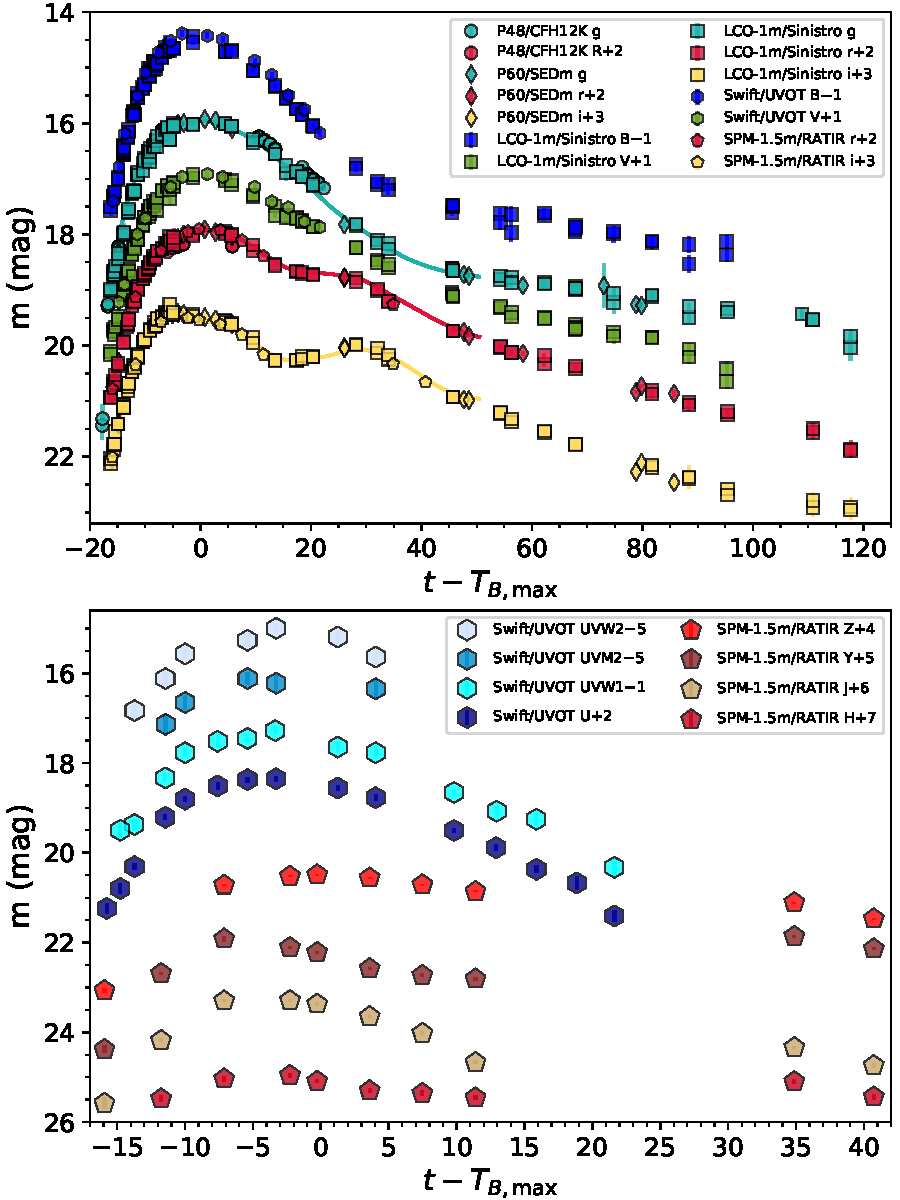
\includegraphics[width=0.95\textwidth]{lightcurve.pdf}
  \caption{Multi-band light curves of iPTF16abc are shown. Filters are
    denoted by different colors and observation instruments by
    different markers. The $t_{max}$ time is the B-band maximum
    determined by SALT2 (Section). The black ticks near the top of the
    figure shows epochs of spectroscopic observations.}
  \label{fig:lightcurve}
\end{figure*}

Spectroscopic observations of iPTF16abc were undertaken with the
Gemini Multi-Object Spectrograph (GMOS; \citealt{2004PASP..116..425H})
on the Gemini North telescope, Low-Resolution Imaging Spectrometer
(LRIS; \citealt{1995PASP..107..375O}) on the Keck-I telescope, DEep
Imaging Multi-Object Spectrograph (DEIMOS;
\citealt{2003SPIE.4841.1657F}) on the Keck-II telescope, The Andalucia
Faint Object Spectrograph and Camera (ALFOSC\footnote{ALFOSC
  instrument webpage:
  \url{http://www.not.iac.es/instruments/alfosc/}}) on the Nordic
Optical Telescope (NOT), and X-shooter \citep{2011A&A...536A.105V} and
Ultraviolet and Visual Echelle Spectrograph (UVES;
\citealt{2000SPIE.4008..534D}) on the Very Large Telescope (VLT). The
observing log is listed in Table \ref{tab:spec_obs_log} and the
low-resolution spectral sequence is shown in Figure
\ref{fig:spec_seq}.

% currently the following table and figure do not include data from LCOGT
\begin{deluxetable*}{cccccc}
  \tablecaption{Spectroscopic observations of iPTF16abc \label{tab:spec_obs_log}}
  \tablehead{
    \colhead{Observation Date} & \colhead{SN phase} & \colhead{Telescope/Instrument} &
    \colhead{Exposure Time (s)} & \colhead{Wavelength Coverage (\AA)} & \colhead{Resolution}
  }
  \startdata
  2016 April $05.88$ & $-15.8$ & Gemini-North/GMOS &     & $3500$ -- $9500$  & $1900$ \\
  2016 April $06.51$ & $-15.1$ & Keck-II/DEIMOS & $1491$ & $5500$ -- $8100$  & $2000$ \\
  2016 April $08.51$ & $-13.1$ & Keck-II/DEIMOS & $900$  & $5500$ -- $8100$  & $2000$ \\
  2016 April $10.38$ & $-11.3$ & Keck-I/LRIS    & $300$  & $3000$ -- $10000$ & $1000$ \\
  2016 April $14.20$ & $-7.5$  & VLT/XSHOOTER   &        & $3000$ -- $25000$ & $10000$ \\
  2016 April $16.??$ & $-5.?$  & VLT/UVES       &        & covers \ion{Ca}{2}\,H$+$K and \ion{Na}{1}\,D lines & $40000$ \\
  2016 April $28.??$ & $6.4$   & NOT/ALFOSC     &        & $3300$ -- $9000$  & $360$ \\
  2016 May   $10.42$ & $18.8$  & Keck-I/LRIS    & $600$  & $3000$ -- $10000$ & $1000$ \\
  2016 May   $12.03$ & $20.4$  & VLT/XSHOOTER   &        & $3000$ -- $25000$ & $10000$ \\
  \enddata
\end{deluxetable*}

\begin{figure*}[htb]
  \centering
  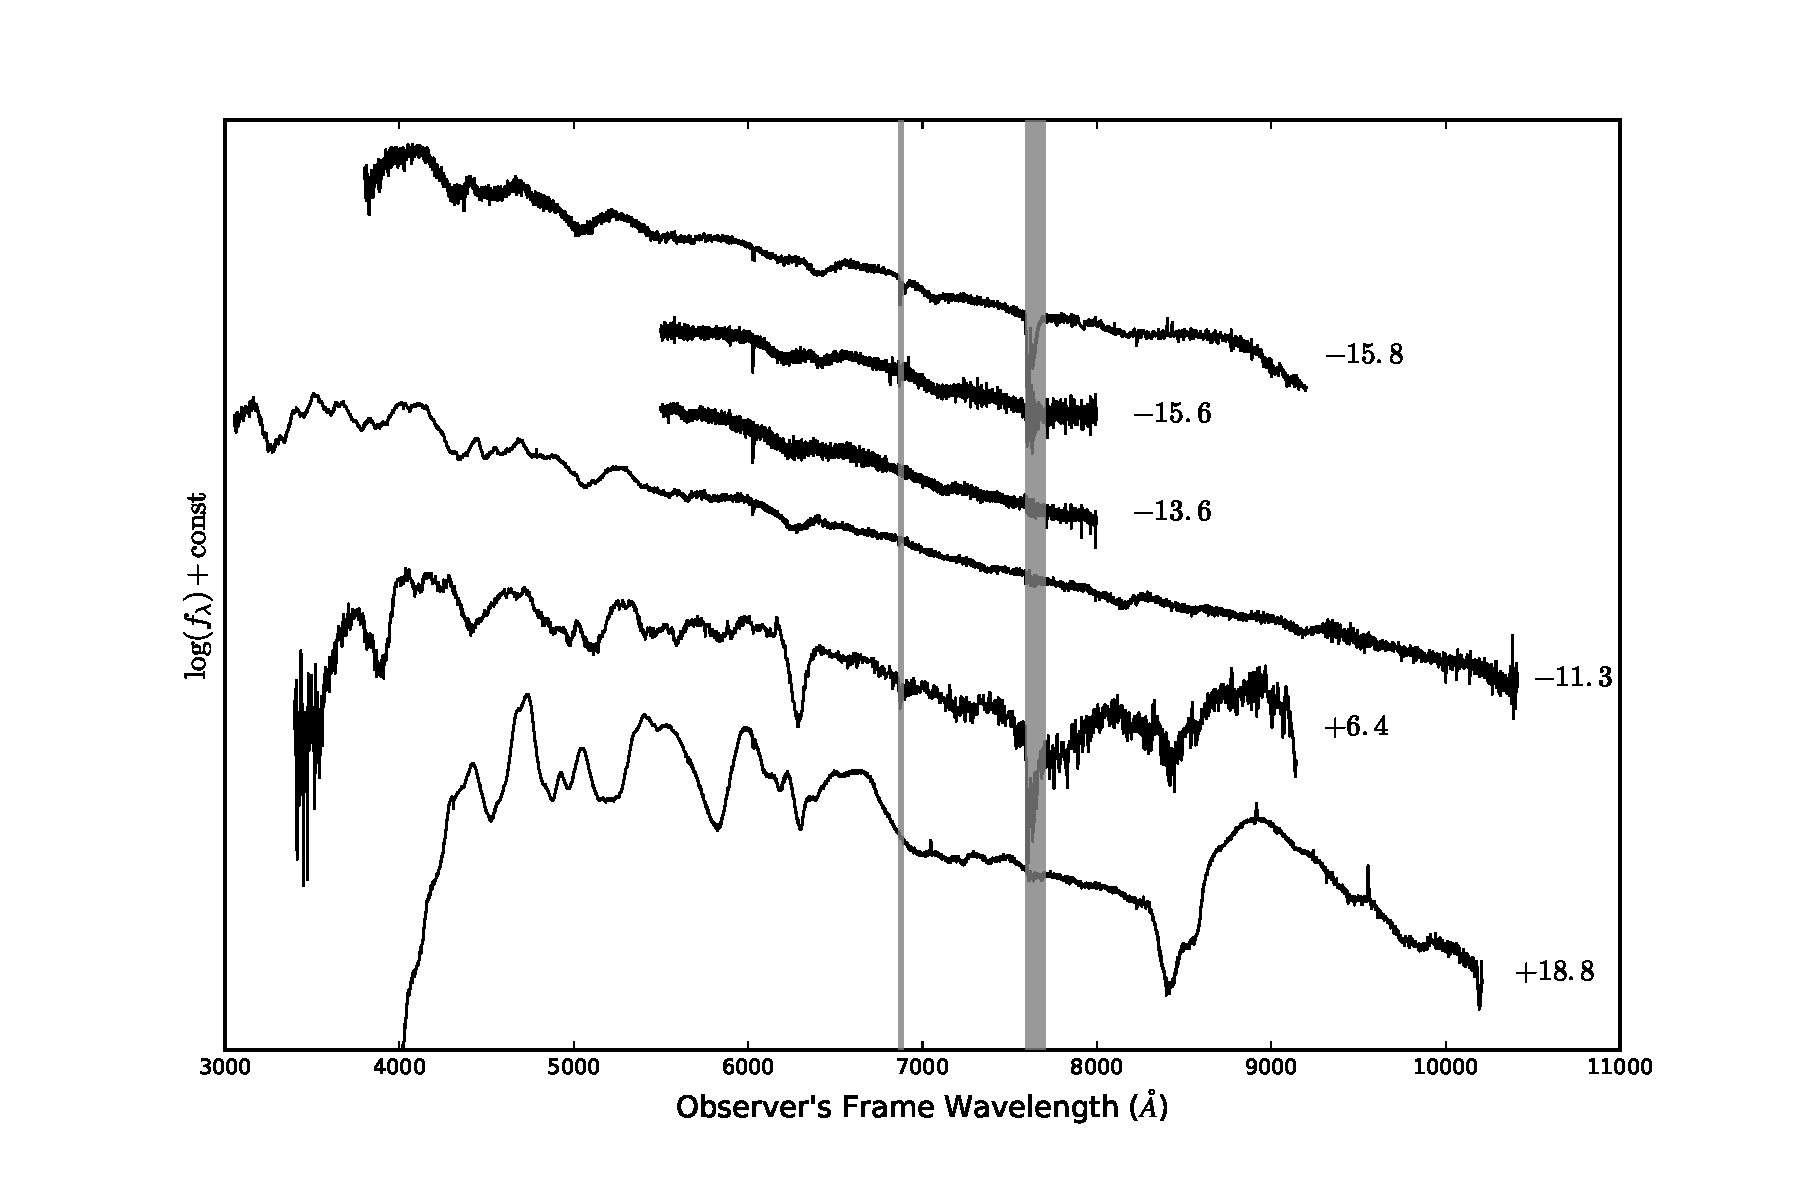
\includegraphics[width=0.9\textwidth]{spec_sequence.pdf}
  \caption{Low-resolution spectra of iPTF16abc are shown in the
    chronical sequence. The phases in units of days are labeled next
    to corresponding spectra. Telluric absorption bands are grayed
    out.}
  \label{fig:spec_seq}
\end{figure*}

\section{Reddening, Classification and Host Galaxy}
\label{sec:usual_staff}

\subsection{Reddening}
\label{sec:reddening}

The foreground Galactic extinctioin along the directionof iPTF16abc ha
$E(B-V)=0.0279\,\textrm{mag}$ \citep{2011ApJ...737..103S}. 

The UVES spectrum of iPTF16abc shows narrow double absorption features
from \ion{Ca}{2}\,H$+$K and \ion{Na}{1}\,D lines (Figure
\ref{fig:narrow_features}), indicating two sources of absorption along
the line of sight. Fitting two Gaussian kernels to each of
the \ion{Na}{1} doublet simultaneously leads to redshifts of
$0.02313820\pm0.00000032$ and $0.02322408\pm0.00000033$. The total
equivalent widths of the \ion{Na}{1}\,D1 and D2 lines are
$0.595\pm0.009\,\textrm{\AA}$ and $0.609\pm0.008\,\textrm{\AA}$.
Using the empirical relation in \citet{2012MNRAS.426.1465P}, we derive
a total extinction of $E(B-V)=0.361\pm0.025\textrm{mag}$.

The X-shooter spectra of iPTF16abc also shows absorption features at
\ion{K}{1}\,7665\,\AA and 7699\,\AA. However, the resolution is not
high enough for the spectra to resolve the two components seen in the
profiles of \ion{Ca}{2} and \ion{Na}{1} in the UVES spectrum. The
X-shooter spectra do not show the diffusive interstellar band at
5780\,\AA as well.  Albeit some arguments (e.g.,
\citealt{2013ApJ...779...38P}), the extinction derived from
\ion{Na}{1}\,D absorption provides the best estimate in the case of
iPTF16abc.

\begin{figure}[htb]
  \centering
  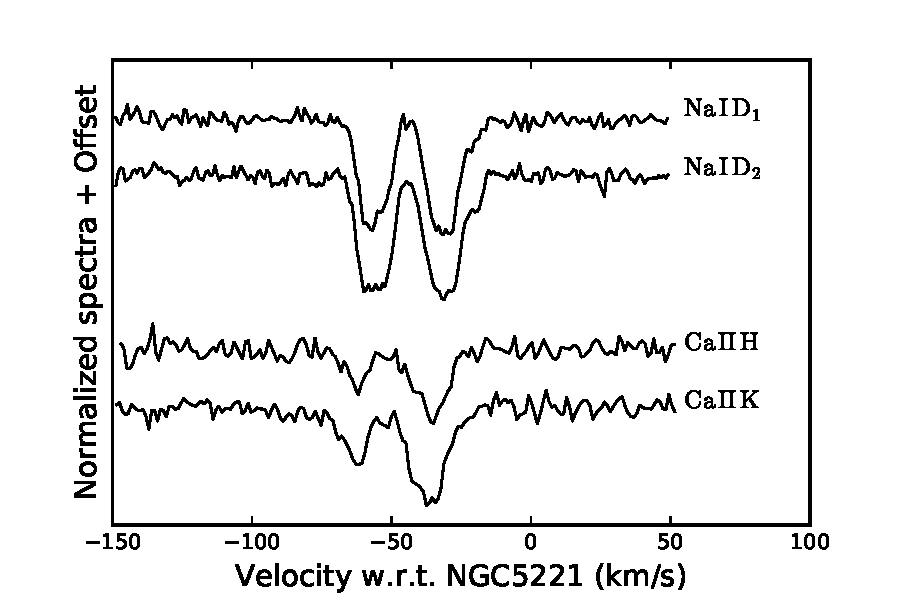
\includegraphics[width=0.45\textwidth]{narrow_abs_features.pdf}
  \caption{Narrow absorption lines of iPTF16abc are shown in this
    figure. The zero velocity corresponds to the redshift of the
    apparent host NGC\,5221.}
  \label{fig:narrow_features}
\end{figure}

The \ion{Na}{1}\,D doublet are resolved in multiple spectra spanning
from pre-peak to post-peak phases. Despite the instrumental widening of
different instrument configurations, we do not detect obvious variation
in the profiles of the doublet.


\subsection{Classfication}
\label{sec:classification}

We run Supernova Identification (SNID; \citealt{2007ApJ...666.1024B})
on the low-resolution spectrum of iPTF16abc at $+18.8$ and found best
matches to normal SNe Ia. Separately the characteristic features of a
SN Ia, such as \ion{Si}{2}, \ion{S}{2}, are obviously seen in the
spectra of iPTF16abc. 

The optical light curves obtained by P48 and P60, after correction for
extinction, are fitted by the SALT2 template
\citep{2007A&A...466...11G} with the \texttt{sncosmo} Python
module\footnote{The \texttt{sncosmo} module is available at
  \url{https://sncosmo.readthedocs.io/en/v1.4.x/}.}. The fitting
parameters are $t_{max}=57499.65\pm0.02$, $x_0=0.0275\pm0.0002$,
$x_1=1.200\pm0.043$, and $c=-0.3353\pm0.0054$. The best-fit model also
gives an unreddened apparent peak magnitude of
$m^*_{B}=14.4\,\textrm{mag}$ in the SN rest frame.

For convenicne, in the following anlaysis and discussion, we define
$t=MJD - 57499.65\,\textrm{days}$, i.e., the time with respect to the
best-fit $t_{max}$. 

\subsection{Host Galaxy}
\label{sec:host}

After establishing iPTF16abc as a normal SN ia, we use the latest
calibration \citep{2014A&A...568A..22B} of the Phillips relation
\citep{1993ApJ...413L.105P} with $m^*_{B}$, $x_1$ and $c$ to derive a
distance modulus $\mu=34.66\pm0.03\,\textrm{mag}$, provided that the
host galaxy of iPTF16abc has a stellar mass less than $10^{10}\sm$.

The location of iPTF16abc is spatially coincident with a tidal tail of
galaxy NGC\,5221. \citet{2007A&A...465...71T} observed this galaxy in
the near-infrared and derived a distance modulus of $35.0\pm0.4\,\textrm{mag}$
from the Tully-Fisher relation. This distance modulus is consistent
with that of iPTF16abc.

Separately, \cite{1998A&AS..130..333T} observed
the 21-cm line in this galaxy and measured a redshift of $0.0233303\pm0.000027$.
The two components in the \ion{Na}{1}\,D have a relative velocity of
$-57.6\pm8.1\,\textrm{km}\,\textrm{s}^{-1}$ and
$-31.8\pm8.1\,\textrm{km}\,\textrm{s}^{-1}$, suggesting that both absorption
resources are probaly located on the tidal tail of NGC\,5221. 


\section{First Light And Early Rise}
\label{sec:early_phases}

In this section, we analyze the early light curve and spectra of iPTF16abc.

\subsection{Light Curve Fit}
\label{sec:lc_fit}

In order to estimate the start time of the observed light curve, denoted as $t_0$,
we fit a power-law model
\begin{equation}
  \label{eq:broken_power_law}
  f(t) \left\{
    \begin{array}{ll}
      = 0,\ \textrm{when}\ t<t_0 \\
      \propto (t-t_0)^{\alpha},\ \textrm{when}\ t>t_0
    \end{array}
  \right.
\end{equation}
to the early-phase \textit{g}-band light curve. We experiment the
fitting procedure with different time windows and find that the light
curve between $t=-18\,\textrm{days}$ and $t=-14\,\textrm{days}$
increases approximately linearly. The best fit model of
$\alpha = 0.97$ and $t_0=-18.47$ is shown in the left panel of
Figure \ref{fig:early_lc_fit} and the join probability distribution of
$\alpha$ and $t_0$ is in the right panel of the same figure.  With the
best-fit $t_0$, our first observation was made only
$0.18\,\textrm{day}$ after the rise of the light curve.

\begin{figure*}[htb]
  \centering
  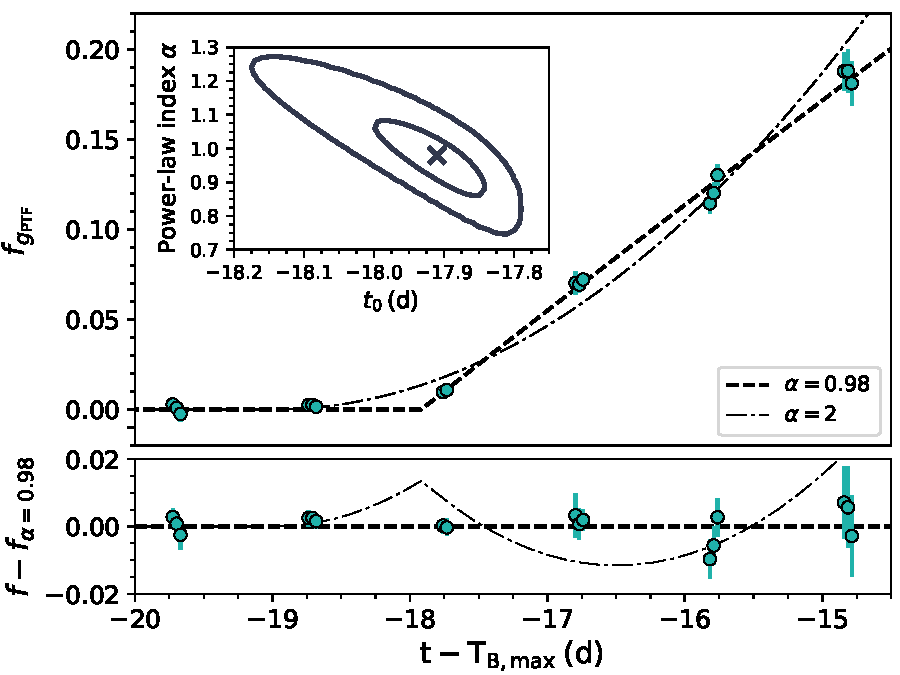
\includegraphics[width=0.45\textwidth]{early_lc.pdf}
  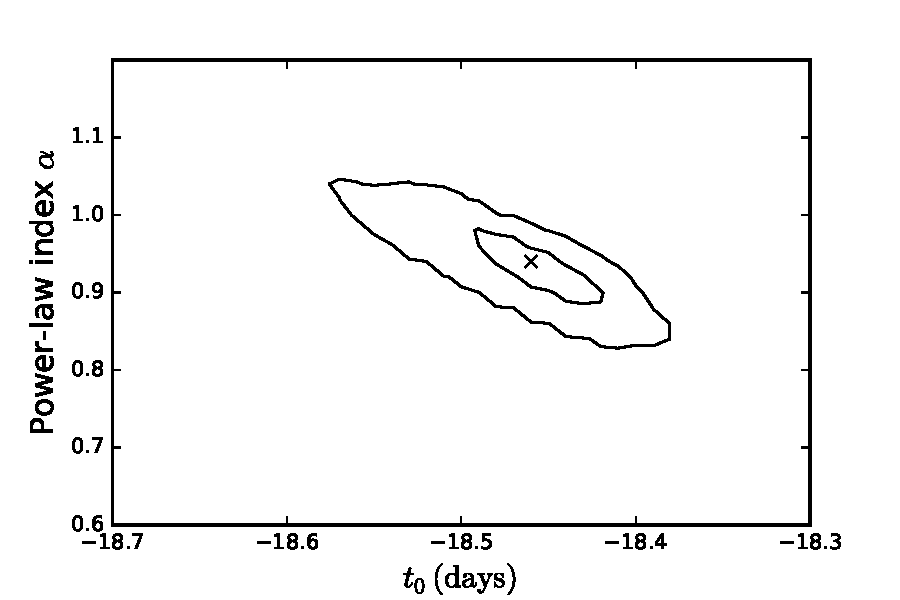
\includegraphics[width=0.45\textwidth]{rise_time_power_law_index.pdf}
  \caption{Broken Power low fitting to the early $g$-band light
    curve. \textit{Left:} the best-fit model of $\alpha=0.94$ and
    $t_0=-18.47\,\textrm{days}$ is illustrated against the
    data. \textit{Right:} the joint distribution of $t_0$ and
    $\alpha$. The cross marker denotes the best-fit parameters. The
    inner and outer contours represent the $68\%$ and $99.7\%$
    confidence levels.}
  \label{fig:early_lc_fit}
\end{figure*}

The \textit{g}-band light curve beyond $t=-14\,\textrm{days}$ rises
significantly faster than the best-fit model above, indicating a
larger value of $\alpha$. In fact, if we fit the light curve between
$t=-14$ and $t=-8$\,days to another power law, we find the best fit at
a power-law index of $1.40$ (Figure \ref{fig:against_sn2012cg}).

Although the early rise behavior of iPTF16abc is distinct from that of
SN2011fe \citep{2011Natur.480..344N} which follows the $t^2$ Arnett
law \citep{1982ApJ...253..785A}, we have seen rise behavior similar to
iPTF16abc (i.e., a steep initial rise followed by a more gradual and
steadier rise) in a few nearby events that were observed at extremely
young phases, such as, SN2013dy \citep{2013ApJ...778L..15Z}, SN2014J
\citep{2014ApJ...783L..24Z}, and ASASSN-14lp
\citep{2016ApJ...826..144S}.

We also note statistical studies on rise
behavior of SNe Ia (e.g., \citealt{2010ApJ...712..350H, 2011MNRAS.416.2607G,
  2012ApJ...745...44G, 2015MNRAS.446.3895F}) which suggest a power-law
index $\gtrapprox2$. However, these studies are not sensitive to SNe Ia
at extremely early phases, so the initial quasi-linear rise of iPTF16abc
is not comparable to their conclusions. On the other hand, the subsequent
$t^{1.40}$ rise of iPTF16abc is roughly consistent with these samples.

\subsection{Expansion Velocity Fit}
\label{sec:early_vel}

As pointed out by \citet{2014ApJ...784...85P}, if a SN light curve is
purely powered by radioactive decay of $^{56}$Ni, the SN may
experience a dark period between the explosion time of the SN
$t_{exp}$ and the rise time of its light curve $t_0$, because it takes
time for radioactive energy to diffuse from where $^{56}$Ni is
deposited in the ejecta and the SN photosphere. Therefore,
\citet{2014ApJ...784...85P} suggests to use the early-phase spectra to
measure line velocities and then estimate $t_{exp}$ by assuming that
$v\propto (t-t_{exp})^{-0.22}$.

We follow the same procedure and
measure the velocities of the \ion{Si}{2}\,6355 line. Because we do
not see signals of multiple velocity components in the
\ion{Si}{2}\,6355 line, and because the \ion{Si}{2}\,6355 line is
partially blended with the \ion{C}{1}\,6580 line, we fit two gaussian
kernels and a linear term simultaneously to spectra between about
6100\,\AA and about 6600\,\AA in the rest frame. Then the velocity is
measured at the minimum of the Gaussian kernel that corresponds to the
\ion{Si}{2} feature.

\begin{figure*}[htb]
  \centering
  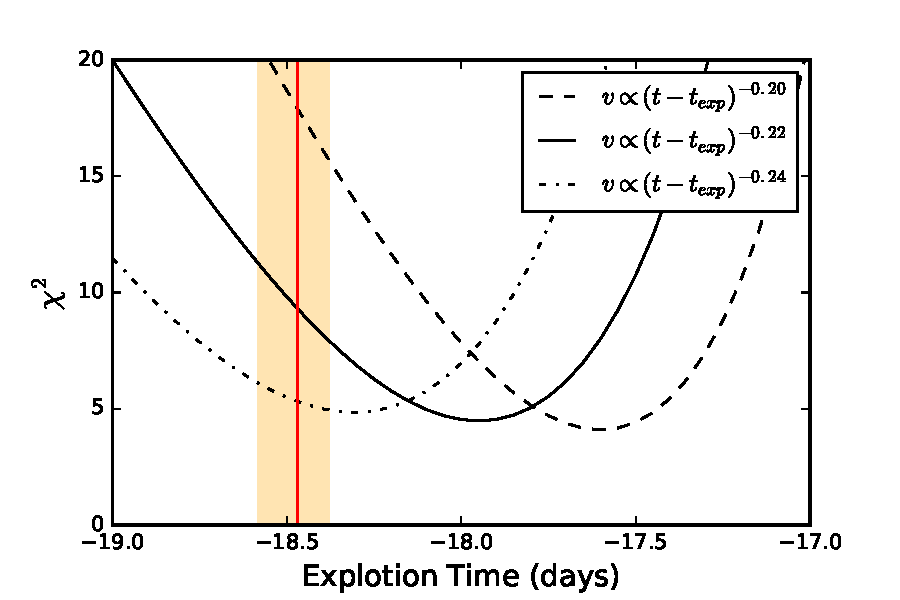
\includegraphics[width=0.45\textwidth]{exp_date_chi2.pdf}
  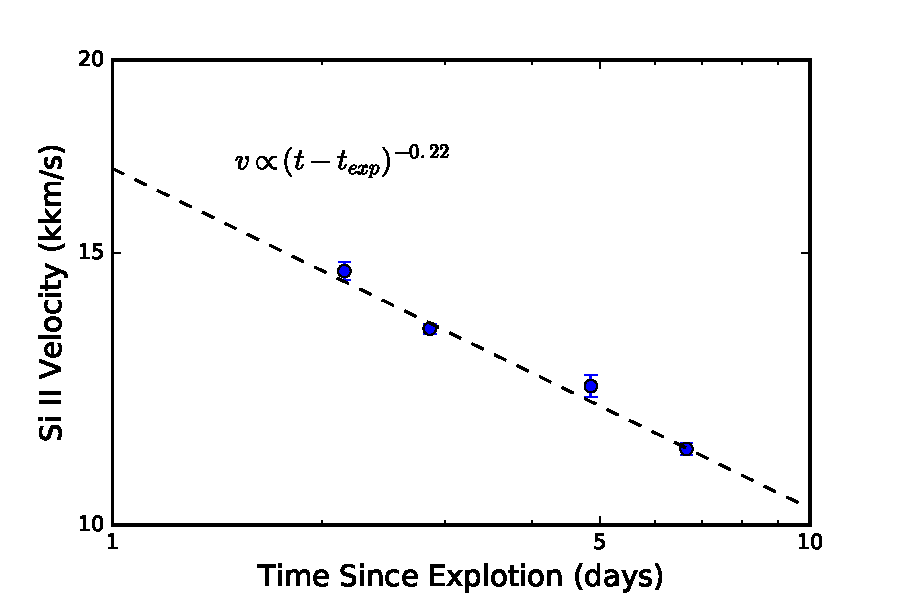
\includegraphics[width=0.45\textwidth]{SiIIVelocity.pdf}
  \caption{Constraints on $t_{exp}$ from fitting the velocity
    evolution of \ion{Si}{2}. \textit{Left panel:} the dashed, solid
    and dash-dotted curves show $\chi^2$ for fitting power laws with
    indices $-0.20$, $-0.22$ and $-0.24$, respectively. The red
    vertical line and the orange region indicate $t_0$ and its
    3-$\sigma$ confidence interval from Section
    \ref{sec:lc_fit}. \textit{Right panel:} Observed \ion{Si}{2}\,6355
    velocities with the best-fit power-law velocity with an index of
    $-0.22$.}
  \label{fig:velocity_t_exp}
\end{figure*}

The expansion velocity fit (Figure \ref{fig:velocity_t_exp}) shows
that the best-fit explosion time $t_{exp}=-17.95\,\textrm{days}$ with
a 3-$\sigma$ confidence interval between $-17.25\,\textrm{days}$ and
$-18.65\,\textrm{days}$.

We further test our assumption $v\propto (t-t_{exp})^{-0.22}$ by
altering the power-law index to $-0.20$ and $-0.24$ (Figure
\ref{fig:velocity_t_exp}).  The best-fit value of $t_0$ varies within
the 3-$\sigma$ confidence interval and the $\chi^2$ value of the
best-fit model varies very little. This test verifies the robustness
of the assumed power-law index of $-0.22$.

Comparing $t_{exp}$ and $t_0$ (Section \ref{sec:lc_fit}), we conclude
that the dark phase of the SN, if exists, is very brief. In the
following analysis, it is reasonable to assume $t_{exp}\simeq t_0$.

\subsection{Light Curve Energy Resources}
\label{sec:lc_energy}

The early portion of a SN light curve may have multiple resources: SN
shockbreakout, SN-companion collision, and radioactive activity. Since
each provides interesting constraints on the progenitor properties, we
explore all the three posibilities.

First, the shock breakout of a SN Ia lasts for a fraction of a second
due to the small size of the exploding star. However, the subsequent
cooling phase may last longer (e.g., \citealt{2010ApJ...708..598P}).
Following the analysis of SN2011fe in \citet{2012ApJ...744L..17B}, we
compare the early-phase \textit{g}-band light curve of iPTF16abc with
two cooling models \citep{2011ApJ...728...63R, 2010ApJ...708..598P}
and reach a not very constraining conclusion that the radius of the
progenitor star of iPTF16abc should be $<1\sr$. In fact, the cooling
emission is negligible at the time of the first detection of iPTF16abc.

Second, if iPTF16abc is born in a single-degenerate channel, with a
chance of $\lesssim10\%$, we expect to see emission produced by SN
ejecta slamming into the companion. In the following we argue from a
statistical \ycao{TBW}

In the case of SN2012cg, \citet{2016ApJ...820...92M} fitted power-law
models to its light curves between $t=-14$ days and $t=-8$ days and
extrapolated backwards to illustrate excess fluxes at $t<-14$
days. The authors further attempted to explain the excess fluxes as
collisional signatures between the SN ejecta and a non-degenerate
companion \citep{2010ApJ...708.1025K}. If we perform the same practice
to the iPTF16abc data, then we find similar excess fluxes at earlier
phases (Figure \ref{fig:against_sn2012cg}). In fact, for any SN whose
light curve can be approximated by a broken-power law, i.e.,
\begin{equation}
  \label{eq:broken-pow}
  f(t) = t^{\alpha}(1 + t^{s(\beta - \alpha)})^{1/s}\ ,
\end{equation}
one can always fit the relative late part of the light curve with a
power law model and find an excess in the early phases.

\begin{figure}[htb]
  \centering
  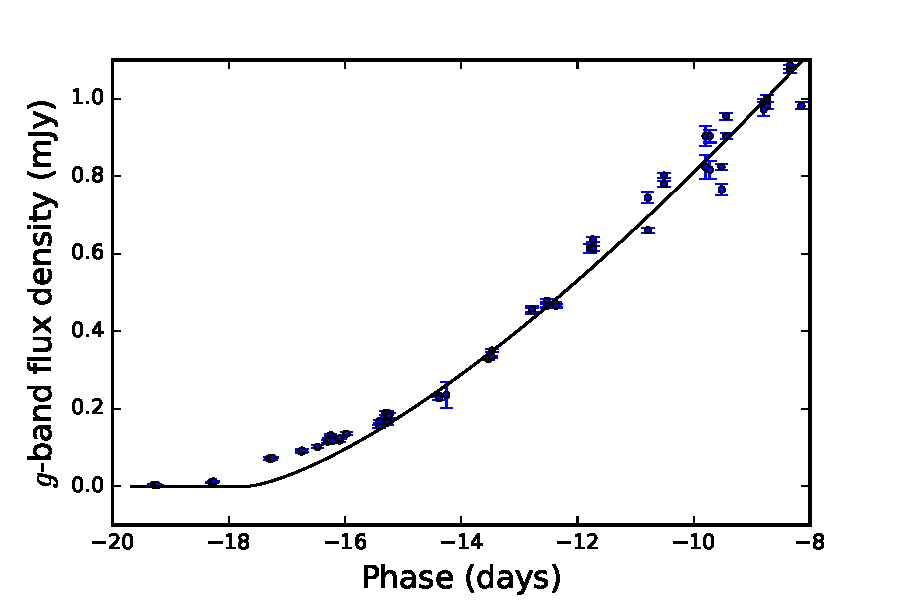
\includegraphics[width=0.45\textwidth]{another_early_lc.pdf}
  \caption{The early-phase \textit{g}-band light curve of iPTF16abc is
    compared against the best-fit power-law model to the data segment
    between $t=-14$ and $t=-8$ days. Note the ``excess'' between the
    data and the model during $t=-18$ and $t=-15$ days}
  \label{fig:against_sn2012cg}
\end{figure}

As a result of the above analysis, we conclude that the early light
curve of iPTF16abc is probably powered dominantly by radioactive decay
of $^{56}$Ni.  According to calculations in
\citet{2016ApJ...826...96P}, when synthesized $^{56}$Ni is mixed
sufficiently in the ejecta, the dark period is short and the initial
light curve rises quickly. In the opposite situation when $^{56}$Ni is
located deeply inside the ejecta, then the dark period can be as long
as a couple days and the initial light curve rises relatively
slowly. The fast initial rise of iPTF16abc and the negligible length
of the dark period both support that $^{56}$Ni is sufficiently mixed
in the ejecta.


\bibliographystyle{aasjournal}
\bibliography{ref}

\end{document}
